\section{Group Key Agreement}

\begin{frame}
\Huge{\centerline{Group Key Agreement (GKA)}}
\end{frame}

\begin{frame}
  \frametitle{GKA}
  GKA constructs a shared secret $\mathcal{K}$. Encryption keys during communication will be derived from $\mathcal{K}$.\\[0.3cm]
  
  Each participant generates a private exponent.  $\mathcal{K}$ will be the shared base raised to all exponents.\\[0.3cm]
  
  For example, for 5 participants with private exponents a, b, c, d and e, and a shared base G:
  \[ \mathcal{K} = G^{abcde} \]

  Any information transmitted is signed using the association table $\mathcal{S}$, so it is:
  \begin{itemize}
    \item Authenticated
    \item Deniable
  \end{itemize}
  
\end{frame}

\begin{frame}
  \frametitle{GKA - Upflow}
  In each step a participant receives an intermediate key list from the previous one, and sends a new intermediate key list to the next one.\\[0.3cm]
  
  The first participant sends a list containing the shared base and the shared base raised to his private exponent.\\[0.3cm]
  
  Each next participant, prepends a copy of the last element to the list, and raises every other element to his private exponent.\\[0.3cm]

  \begin{minipage}{.47\textwidth}
    \[ 1 \rightarrow 2: G, G^a \]
    \[ 2 \rightarrow 3: G^a, G^b, G^{ab} \]
    \[ 3 \rightarrow 4: G^{ab}, G^{ac}, G^{bc}, G^{abc} \]
    \[ 4 \rightarrow 5: G^{abc}, G^{abd}, G^{acd}, G^{bcd}, G^{abcd} \]

  \end{minipage}
  
  \begin{minipage}{.47\textwidth}
   \begin{figure}
      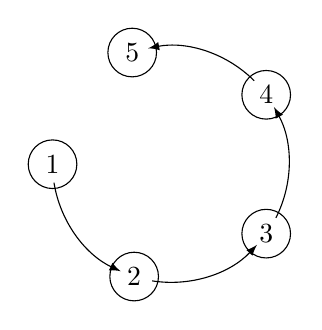
\begin{tikzpicture}[scale=.5]	
        \def \n {5}
        \def \ndec {4}
        \def \radius {3cm}
        \def \margin {8} % margin in angles, depends on the radius

        \foreach \s in {1,...,\ndec}
        {
          \node[draw, circle] at ({180 + (360/\n * (\s - 1))}:\radius) {$\s$};
          \draw[->, >=latex] ({145 + 36 + (360/\n * (\s - 1))+\margin}:\radius)
            arc ({145 + 36 + (360/\n * (\s - 1))+\margin}:{145 + 36 + 360/\n * (\s)-\margin}:\radius);
        }
        \node[draw, circle] at ({181 + 360/\n * (\n - 1)}:\radius) {$\n$};    
      \end{tikzpicture}      
    \end{figure}
  \end{minipage}
\end{frame}

\begin{frame}
  \frametitle{GKA - Downflow}
  Once the last participant has received the upflow, he calculates the shared secret, and broadcasts a new list to all other participants.\\[0.3cm]
  
  He raises every element of the  received list to his private exponent: 
  \[ G^{abce}, G^{abde}, G^{acde}, G^{bcde}, G^{abcde} \]
  
  The last element is $\mathcal{K}$. He saves it and removes it from the list.\\[0.3cm]
  
  Other participants calculate $\mathcal{K}$ by raising the $(n-i)$th element of the list to their private exponent, where n is the length of the list and i their position in the participants order.

  \begin{minipage}{.47\textwidth}
    \[ 5 \rightarrow all: G^{abce}, G^{abde}, G^{acde}, G^{bcde} \]

  \end{minipage}
  
  \begin{minipage}{.47\textwidth}
  \begin{figure}
    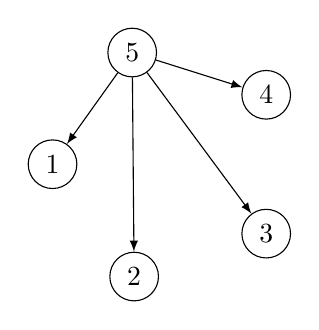
\begin{tikzpicture}[scale=.5]
      \def \n {5}
      \def \ndec {4}
      \def \radius {3cm}
      \def \margin {8} % margin in angles, depends on the radius

      \foreach \s in {1,...,\ndec}
      {
        \node[draw, circle](\s) at ({180 + (360/\n * (\s - 1))}:\radius) {$\s$};
      }
      \node[draw, circle](5) at ({181 + 360/\n * (\n - 1)}:\radius) {$\n$};
      \draw[->, >=latex] (5) -- (1);
      \draw[->, >=latex] (5) -- (2);
      \draw[->, >=latex] (5) -- (3);
      \draw[->, >=latex] (5) -- (4);
    \end{tikzpicture}  
    \end{figure}
  \end{minipage}
\end{frame}